\documentclass[12pt]{article}

% Packages
\usepackage{amsmath, amssymb, mathtools}
\usepackage{graphicx}
\usepackage{physics}
\usepackage{geometry}
\usepackage{enumitem}
\usepackage{bm}
\usepackage{listings}
\usepackage{xcolor}
\usepackage{float}

% Geometry settings
\geometry{letterpaper, margin=1in}
\setlength{\parindent}{0pt}

\definecolor{codegreen}{rgb}{0,0.6,0}
\definecolor{codegray}{rgb}{0.5,0.5,0.5}
\definecolor{codepurple}{rgb}{0.58,0,0.82}
\definecolor{backcolour}{rgb}{0.95,0.95,0.92}

\lstdefinestyle{mystyle}{
    backgroundcolor=\color{backcolour},   
    commentstyle=\color{codegreen},
    keywordstyle=\color{magenta},
    numberstyle=\tiny\color{codegray},
    stringstyle=\color{codepurple},
    basicstyle=\ttfamily\footnotesize,
    breakatwhitespace=false,         
    breaklines=true,                 
    captionpos=b,                    
    keepspaces=true,                 
    numbers=left,                    
    numbersep=5pt,                  
    showspaces=false,                
    showstringspaces=false,
    showtabs=false,                  
    tabsize=2
}

\lstset{style=mystyle}

% Title
\title{Ground-Penetrating Radar Range Profile Estimation}
\author{Sanjot Bains}
\date{\today}

\begin{document}

\maketitle

\section{Introduction}
This report documents the process of reconstructing subsurface range profiles using step-frequency FMCW ground-penetrating radar (GPR) data. The goal is to estimate depth profiles at each antenna position and generate a high-resolution image of the subsurface.

\section{Signal Processing Approach}
\subsection{Data Overview}
The dataset consists of a $128 \times 200$ complex-valued matrix, where each column corresponds to a spatial antenna position (200 total), and each row corresponds to a stepped frequency (128 total, from 0.976~GHz to 2.00~GHz). The spatial step is 0.0213~m, and the relative permittivity of the medium is $\epsilon_r = 6$.

\subsection{Range Estimation Procedure}
\begin{enumerate}[label=(\alph*)]
    \item \textbf{Propagation Speed Adjustment:} The speed of electromagnetic waves in the medium is $v = c/\sqrt{\epsilon_r}$, where $c = 3 \times 10^8$~m/s. This yields $v \approx 1.225 \times 10^8$~m/s.
    \item \textbf{Resolution Calculations:}
    \begin{itemize}
        \item \textit{Bandwidth:} $B = 1$~GHz.
        \item \textit{Time Resolution:} $\Delta t = 1/B = 1$~ns.
        \item \textit{Range Resolution:} $\Delta r = v \Delta t / 2 \approx 0.0612$~m.
        \item \textit{Frequency Resolution:} $\Delta f = (2.00 - 0.976)\,\text{GHz} / 128 \approx 8$~MHz.
        \item \textit{Maximum Time:} $t_{\text{max}} = 1/\Delta f = 125$~ns.
        \item \textit{Maximum Detectable Depth:} $r_{\text{max}} = v t_{\text{max}} / 2 \approx 7.65$~m.
    \end{itemize}
    \item \textbf{Surface Reflection Gating:} Strong reflections near the surface are gated out to improve visualization of subsurface features.
    \item \textbf{Depth Range of Interest:} The rebars are expected at shallow depths ($< 30$~cm), so only the first few pixels in the depth axis are of interest.
\end{enumerate}

\subsection{Interpolation and Image Formation}
\begin{itemize}
    \item \textbf{Depth Interpolation:} Zero-padding the frequency axis to 2048 points increases depth resolution. The IFFT is performed along the frequency axis, and only the last 64 points (corresponding to shallow depths) are retained.
    \item \textbf{Lateral Interpolation:} The spatial axis is padded to 256 points, FFT is performed, and then zero-padded to 2048 points in the frequency domain. An IFFT yields a finely sampled lateral profile.
    \item \textbf{Physical Pixel Size:} After interpolation, the depth pixel size is $0.3827$~cm, and the lateral pixel size is $0.26625$~cm.
\end{itemize}

\section{Resolution and Maximum Detectable Depth}
\begin{itemize}
    \item \textbf{Range (Depth) Resolution:} $\Delta r = 0.0612$~m ($6.12$~cm) before interpolation; after zero-padding, the effective pixel size is $0.3827$~cm.
    \item \textbf{Maximum Detectable Depth:} $r_{\text{max}} \approx 7.65$~m.
\end{itemize}

\section{Physical Pixel Size}
\begin{itemize}
    \item \textbf{Depth Direction:} $0.3827$~cm per pixel (after zero-padding and IFFT).
    \item \textbf{Lateral Direction:} $0.26625$~cm per pixel (after zero-padding and IFFT).
\end{itemize}

\section{Final Image}
\begin{figure}[H]
    \centering
    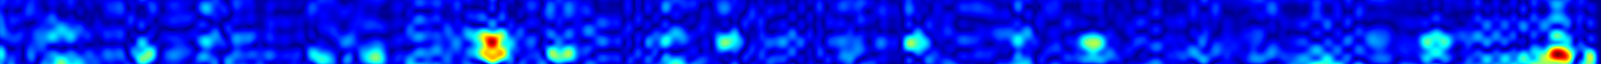
\includegraphics[width=1.0\textwidth]{depth_map.png}
    \caption{Final interpolated range profile image. The vertical axis represents depth (shallowest at the top), and the horizontal axis represents antenna position along the scan path.}
\end{figure}

\section{Code}
\begin{lstlisting}[language=Octave, caption=Ground-Penetrating Radar Range Profile Estimation]
gpr_data = load('gpr_data/gpr_data.mat');

F = gpr_data.F; 
f = gpr_data.f;
da = gpr_data.da;

epsilon_r = 6;

c = 3 * 10^8; # m/s 
velocity = c / sqrt(epsilon_r); # = 1.2247e+08 m/s

bandwidth = 1 * 10^9; % 1 GHz

% Time Resolution
delta_t = 1 / bandwidth; % 10^-9 s

% Range Resolution
delta_r = velocity * delta_t / 2; % = 0.061237 m

% Frequency Resolution
delta_f = (2 - 0.976) * 10^9 / 128; % = 8 MHz

% Max Time 
range_time_max = 1 / delta_f; % = 1.25 * 10^-7 s

% Max Distance
range_distance_max = velocity * range_time_max / 2; % = 7.6547 m

% Dividing 765 cm / 24 cm (within our range of interest), yields approximately
% 32.

% We have 128 frequencies: 128/32 = 4, meaning we only care about the first 4 px.

%% INTERPOLATION

%% Interpolating Range (Depth) for Display (Columns)

% THE SIZE OF OUR DATA IS 128 columns x 200 rows.

% We want to interpolate the depth data to 2048 points.
% Interpolation factor = 2048 / 128 = 16

% We need to zero-pad the data to 2048 points.
% Very naively, we can just pad with zeros at the end of each column.
% We know the freq resolution is 8 Mhz, and the minimum frequency is 0.976 GHz.
% That means we can determine the number of empty points we should add infront
% of the data.

pts_front = 0.976 * 10^9 / delta_f; % = 122
F_padded = zeros(2048, 200);
F_padded(pts_front + 1 : pts_front + 128, :) = F;

% THE SIZE OF OUR DATA IS 2048 rows x 200 columns.

F_ifft = ifft(F_padded, [], 1);

% The IFFT turns the columnar frequency data into depth profiles.

F_ifft = ifft(F_padded, [], 1)(1985:2048, :);
    % Number of pixels for display = (4*16) = 64
    % Pixel size = 6.1237 cm / 16 = 0.3827 cm

% THE SIZE OF OUR DATA IS 64 rows x 200 columns.

%% Interpolating receiver positions. (horizontal)

% We have 200 receiver positions

% We will first pad by 28 zeros at the beginning and end of the receiver pos axis.
% This lets us FFT the data.
F_padded = zeros(64, 256);
F_padded(:, 29:228) = F_ifft;

# THE SIZE OF OUR DATA IS 64 rows x 256 columns.

% Now we can perform the FFT along the position axis.
F_fft = fft(F_padded, [], 2);

% In the frequency domain we can zero pad the position data to 2048 points.
% We add zeros to the middle of the data
F_padded = zeros(64, 2048);
F_padded(:, 1:128) = F_fft(:, 1:128);
F_padded(:, 1921:2048) = F_fft(:, 129:256);

# THE SIZE OF OUR DATA IS 64 rows x 2048 columns.

% Perform the IFFT on the padded data
F_ifft = ifft(F_padded, [], 2);

% We are now back in the spatial domain, with 2048 receiver points.
% The interpolation ratio is 2048/256 = 8.
% The pixel size is 0.0213 m / 8 = 0.0026625 m = 2.6625 mm = 0.26625 cm

% To get a properly scaled image we must take into account the disparate
% pixel sizes in the depth and horizontal directions.

% Each depth pixel is 0.3827 cm, and each horizontal pixel is 0.26625 cm.

img = abs(F_ifft)(:, 225:1825);
img = img - min(img(:));
img = img / max(img(:));
img_uint8 = uint8(img * 255);
cmap = jet(256);
imwrite(img_uint8, cmap, 'depth_map.png');

\end{lstlisting}

\section{Summary}
\begin{itemize}
    \item The GPR data was processed using FFT and IFFT techniques to estimate subsurface range profiles.
    \item Zero-padding in both frequency and spatial domains enabled high-resolution interpolation, yielding a final image with sub-centimeter pixel sizes.
    \item The depth resolution is $0.3827$~cm, and the maximum detectable depth is $7.65$~m, though only shallow depths are of practical interest.
    \item The final image clearly visualizes subsurface features, such as rebars, with high spatial and depth resolution.
    \item I was not able to get the contrast of the example image. I am dealing with an unfamiliar programming suite, but that's not really an excuse.
\end{itemize}

\end{document}